\documentclass[german,12pt]{homework}

\usepackage[ngerman]{babel}
\usepackage[utf8]{inputenc}
\usepackage[T1]{fontenc}

\usepackage{graphicx}
\graphicspath{ {./images/} }

\usepackage{tikz}
\usetikzlibrary{calc,angles,quotes,babel}

\usepackage{amsmath}
\usepackage{mathtools}
\usepackage{amssymb}
\usepackage{icomma}

\makeatletter
\def\underbarvec#1{\underline{\sbox\tw@{$#1$}\dp\tw@\z@\box\tw@}}
\makeatother

\DeclarePairedDelimiter{\absolute}{\lvert}{\rvert}
\DeclarePairedDelimiter{\enbrace}{(}{)}
\DeclarePairedDelimiter{\benbrace}{[}{]}

\usepackage{chemformula}
\usepackage{siunitx}
\newcommand{\sis}[1]{\,\si{#1}}
\newcommand{\degC}{\si{\degreeCelsius}}

\sisetup{per-mode=fraction,sticky-per}

\title{Vorrechenübung 1}
\author{Joshua Feld, 406718}
\institute{RWTH Aachen University\\Lehrstuhl für computergestützte Analyse
technischer Systeme}
\class{Mechanik I}
\professor{Prof. Dr. Behr}

\begin{document}
    \maketitle

    \section*{Aufgabe 1. (Kinetische Energie)}

    \begin{problem}
        Wenn sich ein starrer Körper der Masse \(m\) in der Ebene bewegt, wird seine kinetische Energie (\(E_k\)) über die Gleichung
        \[E_k = \frac{1}{2}mv^2 + \frac{1}{2}mk^2\omega^2\]
        beschrieben. Hierbei sind \(v\) die Geschwindigkeit am Schwerpunkt, \(k\) eine Konstante und \(\omega\) die Winkelgeschwindigkeit des Körpers (Einheit \(\benbrace*{T}^{-1}\)). Bestimmen Sie die Einheiten von \(E_k\) und \(k\) im \(\benbrace*{MLT}\)-System.
    \end{problem}

    \subsection*{Lösung} Die folgenden Einheiten sind bekannt:
    \[\benbrace*{m} = \benbrace*{M}, \quad \benbrace*{v} = \benbrace*{\frac{L}{T}}, \quad \benbrace*{\omega} = \benbrace*{\frac{1}{T}}.\]
    Betrachten wir zunächst nur den ersten Teil der Gleichung, also \(\frac{1}{2}mv^2\). Dafür ergibt sich dann direkt
    \[\benbrace*{E_k} = \benbrace*{m}\benbrace*{v}^2 + \ldots = \benbrace*{M}\benbrace*{\frac{L}{T}}^2 = \benbrace*{M\frac{L^2}{T^2}}\]
    Nun betrachten wir den zweiten Teil:
    \[\benbrace*{E_k} = \ldots + \benbrace*{m}\benbrace*{k}^2\benbrace*{\omega}^2 \iff \benbrace*{M\frac{L^2}{T^2}} = \benbrace*{M}\benbrace*{k}^2\benbrace*{\frac{1}{T}}^2 \iff \benbrace*{k}^2 = \benbrace*{L}^2 \iff \benbrace*{k} = \benbrace*{L}\]

    \section*{Aufgabe 2. (Traktoren)}

    \begin{problem}
        Ein Baumstamm wird von zwei Traktoren \(A\) und \(B\) gezogen. Bestimme den Betrag und die Richtung der beiden Zugkräfte \(F_A\) und \(F_B\). Die resultierende Kraft soll entlang der \(x\)-Achse wirken. Gegeben ist \(F_R = 10\sis{\kilo\newton}\), \(\theta = 15^\circ\) und \(\alpha = 30^\circ\).

        \begin{center}
            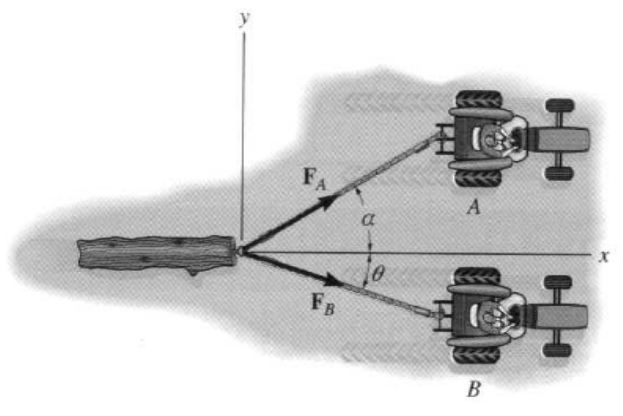
\includegraphics[scale=.4]{traktoren}
        \end{center}
    \end{problem}

    \subsection*{Lösung} Aus der Aufgabenstellung erhalten wir \(F_R = \absolute*{F_R} = 10\sis{\kilo\newton}\), \(\theta = 15^{\circ}\) und \(\alpha = 30^{\circ}\). Wir wollen nun die Kräfte, die durch die Vektoren erzeugt werden, \(\underbarvec{F}_A\) und \(\underbarvec{F}_B\), berechnen. Wir kennen die resultierende Kraft, also gilt \(\underbarvec{F}_R = \underbarvec{F}_A + \underbarvec{F}_B\). Wir betrachten nun eine Skizze:
    \begin{center}
        \begin{tikzpicture}
            \coordinate (o) at (0,0);
            \coordinate (a) at (2,2);
            \coordinate (b) at (5,0);

            \draw [->] (0,0) -- (5.5,0) node[below] {\(x\)};
            \draw [->] (0,0) -- (0,3) node[right] {\(y\)};
            \draw [->,thick] (0,0) -- (5,0) node [midway,below] {\(\underbarvec{F}_R\)};
            \draw [->] (0,0) -- (2,2) node [midway,above,sloped] {\(\underbarvec{F}_A\)};
            \draw [->] (2,2) -- (5,0) node [midway,above,sloped] {\(\underbarvec{F}_B\)};
            \draw [->,dashed] (0,0) -- (3,-2);
            \draw [->,dashed] (3,-2) -- (5,0);

            \pic[draw, "$\alpha$",-, angle eccentricity=1.5] {angle=b--o--a};
            \pic[draw, "$\beta$", -, angle eccentricity=1.6] {angle=o--a--b};
            \pic[draw, "$\theta$",-, angle eccentricity=1.5] {angle=a--b--o};
        \end{tikzpicture}
    \end{center}
    Nach dem aus der Vorlesung bekannten Sinussatz gilt
    \[\frac{F_R}{\sin\beta} = \frac{F_A}{\sin\theta} = \frac{F_B}{\sin\alpha},\]
    also \(\underbarvec{F}_A = \underbarvec{F}_R\frac{\sin\theta}{\sin\beta} = 3,66\sis{\kilo\newton}\) und \(\underbarvec{F}_B = \underbarvec{F}_R\frac{\sin\alpha}{\sin\beta} = 7,07\sis{\kilo\newton}\). Wir müssen nun noch die Richtung der Kräfte bestimmen. Im Allgemeinen gilt für einen Kraftvektor \(\underbarvec{A} = \absolute*{\underbarvec{A}} \cdot \underbarvec{\lambda}_A\), mit \(\absolute*{\underbarvec{\lambda}_A} = 1\); in unserem Fall also \(\underbarvec{F}_A = \absolute*{\underbarvec{F}_A} \cdot \underbarvec{\lambda}_A\) und \(\underbarvec{F}_B = \absolute*{\underbarvec{F}_B} \cdot \underbarvec{\lambda}_B\). Es gilt
    \[\cos\alpha = \frac{\lambda_{Ax}}{\absolute*{\underbarvec{\lambda}_A}} \iff \lambda_{Ax} = \underbrace{\absolute*{\underbarvec{\lambda}_A}}_{= 1} \cdot \cos\alpha = \cos\alpha = \cos 30^\circ,\]
    \[\sin\alpha = \frac{\lambda_{Ay}}{\absolute*{\underbarvec{\lambda}_A}} \iff \lambda_{Ay} = \absolute*{\underbarvec{\lambda}_A} \cdot \sin\alpha = \sin\alpha = \sin 30^\circ,\]
    also \(\underbarvec{F}_A = F_A\begin{pmatrix}\cos 30^\circ\\\sin 30^\circ\end{pmatrix}\) und
    \[\cos\theta = \frac{\lambda_{Bx}}{\absolute*{\underbarvec{\lambda}_B}} \iff \lambda_{Bx} = \underbrace{\absolute*{\underbarvec{\lambda}_B}}_{= 1} \cdot \cos\theta = \cos\theta = \cos 15^\circ,\]
    \[\sin\theta = \frac{\lambda_{By}}{\absolute*{\underbarvec{\lambda}_B}} \iff \lambda_{By} = \absolute*{\underbarvec{\lambda}_B} \cdot \sin\theta = \sin\theta = \sin 15^\circ,\]
    also \(\underbarvec{F}_B = F_B\begin{pmatrix}\cos 15^\circ\\\sin 15^\circ\end{pmatrix}\). Dies können wir nun noch überprüfen mithilfe der Vektoraddition von \(\underbarvec{F}_A\) und \(\underbarvec{F}_B\):
    \[\underbarvec{F}_R = \underbarvec{F}_A + \underbarvec{F}_B = F_A\begin{pmatrix}\cos 30^\circ\\\sin 30^\circ\end{pmatrix} + F_B\begin{pmatrix}\cos 15^\circ\\\sin 15^\circ\end{pmatrix} = \begin{pmatrix}10\sis{\kilo\newton}\\0\sis{\kilo\newton}\end{pmatrix}.\]
\end{document}
